\documentclass[12pt]{article}

% More detailed margin control
\usepackage[left=1in,right=1in,top=1in,bottom=1in]{geometry}

% Essential packages
\usepackage{amsmath}
\usepackage[utf8]{inputenc} % allow utf-8 input
\usepackage[T1]{fontenc}    % use 8-bit T1 fonts
\usepackage{lmodern}
\usepackage{hyperref}       % hyperlinks
\usepackage{url}            % simple URL typesetting
\usepackage{booktabs}       % professional-quality tables
\usepackage{amsfonts}       % blackboard math symbols
\usepackage{nicefrac}       % compact symbols for 1/2, etc.
\usepackage{microtype}      % microtypography
\usepackage{xcolor}         % colors
\usepackage{comment}
\usepackage{enumitem}
\usepackage[ruled,vlined]{algorithm2e}
\usepackage{algpseudocode}
\usepackage{subcaption}
\usepackage{graphicx}
\usepackage{tikz}
\usetikzlibrary{shapes, arrows.meta, positioning, fit}
\usepackage{amsthm}
\usepackage[backend=biber, style=apa]{biblatex}


\usepackage{nicefrac}       % compact symbols for 1/2, etc.


% Compatibility for biblatex
\usepackage{csquotes}

% Load biblatex before cleveref
\usepackage{biblatex}

\usepackage{cleveref}
\addbibresource{references.bib}
% Define custom commands if not already defined
\newcommand{\EE}{\mathbb{E}}
\newcommand{\R}{\mathbb{R}}

% Theorem environments
\newtheorem{assumption}{Assumption}
\newtheorem{lemma}{Lemma}
\newtheorem{proposition}{Proposition}
\newtheorem{theorem}{Theorem}
\newtheorem{corollary}{Corollary}
\newtheorem{definition}{Definition}
\newtheorem{remark}{Remark}

% Comments for co-authors (optional)
\newcommand{\coauthorcomment}[2]{{\color{#1} \textbf{#2}}}

\usepackage{xspace}
\newcommand{\algname}[1]{{\sf  #1}\xspace}
\newcommand{\algnamex}[1]{{\sf #1}\xspace}

% Title and author information
\title{LLMs Consistency in Describing and Scoring Personality}

\author{
  Danila Chernousov\\
}

\begin{document}

\maketitle

\begin{abstract}
In this paper, we propose a novel approach for evaluating Large Language Models' ability to be profiled with a simple prompt containing a set of scores along several personality dimensions. We assess LLM consistency in both describing and scoring personality traits through a two-stage experiment. We show that when asked explicitly, LLMs can convert numerical scores to text and back consistently. Our framework evaluates LLM consistency not only on well-established traits (e.g., Big Five) but also on understudied or synthetic trait combinations. We find that LLMs exhibit higher consistency for widely studied traits compared to under-researched or ambiguous constructs.


\end{abstract}

\paragraph{Keywords:} AI Agents, Large Language Model, Agent-Based Simulation, Agent Profiling, LLM consistency.

\section{Introduction}

Large language models (LLMs) have been rapidly integrated into applications that require human-like interaction—such as virtual assistants or therapeutic chatbots [\cite{sun2024random}, \cite{argyle2023out}, \cite{park2023generative}] — fueling interest in their ability to simulate consistent, personalized behavior. Argyle et al. introduced the idea of silicone sampling, enabling LLMs to represent human populations in downstream tasks [\cite{argyle2023out}, \cite{santurkar2023whose}, \cite{manning2024automated}, \cite{jiang2023evaluating}, \cite{serapio2023personality}], while [\cite{horton2023large}, \cite{leng2024can}, \cite{jiang2023personallm}]. demonstrated that LLMs reflect many of the same biases observed in human decision-making. 
If we imagine personality as a point in a vector space, we can choose basis vectors, such as openness, extraversion, and agreeableness and profile agents along these dimensions. In theory, this allows for precise control over agent behavior using a small set of trait values. However, before employing arbitrary or task-specific trait sets, we must be certain that an LLM both understands such profiling and behaves within the confines of the specified personality. A core challenge in agent profiling is configuring LLMs to adopt target personality traits, values, or behavioral patterns purely through prompts, without relying on long-term memory or fine-tuning.

Although recent work has explored the capacity of LLMs to mimic human personalities, a critical question remains understudied: \textit{consistency} — the degree to which an agent simulates the behavior of a personality with which it was profiled. Existing research [\cite{frisch2024llm}, \cite{tommaso2024llms}, \cite{shu2023you}, \cite{song2023have} \cite{jiang2023personallm}, \cite{gupta2023self}] indicates that LLMs do not possess any personality by themselves and thus are not consistent (for example, their answers depend on the order in which they were presented to them). Yet, existing evaluations have largely focused on alignment with established psychometric frameworks like the Big Five Inventory (BFI) - most popular psychometric scale, consisting of 5 traits: Openness, Conscientiousness, Extraversion, Agreeableness, and Neuroticism (OCEAN). These approaches share two key limitations:

    \textbf{Memorized Associations}: They rely on well-documented traits—e.g., extraversion or neuroticism—for which LLMs have abundant training data, potentially conflating true consistency with learned textual correlations.

    \textbf{Limited Scope}: Restricting analysis to predefined human-centric taxonomies precludes assessment of synthetic or understudied trait combinations (e.g., “risk-seeking vs. deliberative” or “aesthetic sensitivity”), leaving gaps in our understanding of LLMs’ general profiling capabilities.

To address these gaps, we introduce a two-stage, cross-session methodology that evaluates LLMs' intrinsic consistency in translating between numerical personality scores and textual descriptions—and back again—without relying on contextual memory. In the first stage, the model receives a prompt containing specific trait scores and generates an implicit description of an agent’s personality. In the second stage, the same model is tasked with inferring numerical scores based solely on that description. Each stage occurs in a separate chat session, ensuring no hidden memory of previous inputs. By comparing original and inferred scores, we directly measure the model’s consistency in both describing and interpreting personality traits.

This framework functions as an intrinsic benchmark of an LLM's ability to convert structured personality information (i.e., numerical scores) into a coherent, text-based persona, and to reverse this process when prompted. It also allows us to test the limits of LLM flexibility across both well-established and non-canonical dimensions.

Applying our framework to both canonical (e.g., Big Five) and novel trait sets, we find that LLMs exhibit higher consistency for widely studied traits. Additionaly, we show that consistency depends on the ordering of traits. These results highlight a tension between LLMs’ flexible role-playing capabilities and their dependence on patterns embedded in training data.


All of the code used can be found at the github page. \footnote{https://github.com/Chernousovdv/Personalized-AI-Agent}
\section{Problem Statement}

\begin{figure}[htbp]
  \centering
  \begin{document}
\begin{tikzpicture}[
    node distance=1cm,  % Reduced general spacing
    box/.style={rectangle, draw, rounded corners, minimum width=2cm, minimum height=1cm, align=center},
    agent/.style={box, trapezium, trapezium left angle=70, trapezium right angle=110},
    arrow/.style={-Stealth, thick},
    trait/.style={circle, draw=red, fill=red!20, thick, minimum size=0.7cm, font=\small}
]

% Personality Trait Labels
\node[] (label1) at (-2,0) {Openness};
\node[] (label2) at (-2,-1.6) {Extraversion};
\node[] (label3) at (-2,-3.2) {Agreeableness};

% Enclosing box for trait labels
\node[draw, rounded corners, inner sep=0.1cm, fit=(label1) (label3), label=above:Traits] (traitbox) {};

% Personality Scores (vertical circles)
\node[trait] (trait1) at (0,0) {4};
\node[trait, below=0.8cm of trait1] (trait2) {3};
\node[trait, below=0.8cm of trait2] (trait3) {5};

% Enclosing box for scores
\node[draw, rounded corners, inner sep=0.2cm, fit=(trait1) (trait3), label=above:Scores] (scores) {};

% Rest of the nodes with tighter spacing
\node[agent, right=1.5cm of scores] (agent1) {
\includegraphics[height=0.5cm]{openai.jpeg}\\Agent 1};
\node[box, right=1.5cm of agent1] (text) {Text\\Description};
\node[agent, right=1.5cm of text] (agent2) {
\includegraphics[height=0.5cm]{openai.jpeg}\\Agent 2};

% Generated Scores - positioned with shorter distance
\node[trait, right=1.5cm of agent2] (gen1) {4.2};
\node[trait, below=0.8cm of gen1] (gen2) {2.8};
\node[trait, above=0.8cm of gen1] (gen3) {4.9};
\node[draw, rounded corners, inner sep=0.2cm, fit=(gen2) (gen3), label=above:Generated Scores] (generated) {};

\node[box, below=1.5cm of text] (cosine) {MAE};

% Shorter main flow arrows
\draw[arrow] (scores.east) -- (agent1.west);
\draw[arrow] (agent1) -- (text);
\draw[arrow] (text) -- (agent2);
\draw[arrow] (agent2) -- (generated.west);

% Comparison arrows
\draw[arrow] (scores.south) -- (cosine.west);
\draw[arrow] (generated.south) -- (cosine.east);

% Labels

\end{tikzpicture}
\end{document} % Path to your .tex file
  \caption{Experiment pipeline. We prompt Agent1 to generate text description. Agent2 generates scores based on the text description without seeing original scores}
  \label{fig:personality}
\end{figure}

The problem can be formulated as follows:

\begin{center}
    \textbf{Can LLMs be consistent in personality scoring?}
\end{center}

To explain this idea further we will use mathematical notation

Let $\mathbf{p} \in \mathcal{P} \subset \mathbb{R}^n$ represent a personality trait vector in an $n$-dimensional space, and $\mathcal{D}$ denote the space of textual descriptions. We consider two mappings:

\begin{equation}
    f: \mathcal{P} \to \mathcal{D}, \quad f(\mathbf{p}) = \mathbf{d} \quad \text{(trait-to-text encoding)}
\end{equation}

\begin{equation}
    g: \mathcal{D} \to \mathcal{P}, \quad g(\mathbf{d}) = \mathbf{p'} \quad \text{(text-to-trait decoding)}
\end{equation}

The core problem is to evaluate whether the composition $g \circ f$ preserves personality vectors with minimal distortion:
\begin{equation}
    \|\mathbf{p} - g(f(\mathbf{p}))\| < \epsilon \quad \forall \mathbf{p} \in \mathcal{P},
\end{equation}
where $\epsilon$ is an acceptable error threshold. Specifically:

\begin{itemize}
    \item Do LLMs implement $f$ and $g$ such that reconstructed vectors $\mathbf{p'}$ remain $\epsilon$-close to originals $\mathbf{p}$?
    \item Does the error $\|\mathbf{p} - \mathbf{p'}\|$ increase for subspaces $\mathcal{S} \subset \mathcal{P}$ with limited training data coverage?
\end{itemize}

This quantifies whether LLMs can reliably serve as lossless translators between numeric personality representations and their textual embeddings - a fundamental requirement for stable AI agent design.

\section{Theory}

We use the following algorithm for each set of traits. The traits we chose are discussed in the next section



\begin{algorithm}[H]
\caption{LLM Personality Consistency Evaluation}
\KwIn{Personality traits $\mathcal{T}$, True scores $S_{true}$, Number of trials $N$}
\KwOut{Consistency metrics $M$}

\SetAlgoLined
\DontPrintSemicolon


\For{$i \gets 1$ \textbf{to} $N$}{
    $D_i \gets \Call{GenerateDescription}{\mathcal{T}, S_{true}}$\;
    
    $S_{recon} \gets \Call{ExtractScores}{D_i, \mathcal{T}}$\;
    
    \For{$\tau \in \mathcal{T}$}{
        $M_i[\tau] \gets |S_{true}[\tau] - S_{recon}[\tau]|$\;
    }
    $\Call{UpdateMetrics}{M, M_i}$\;
}

$M_{mae} \gets \Call{MeanAbsoluteError}{M}$\;

\Return $M_{mae}$\;


\end{algorithm}


\section{Role of Temperature in Generating Descriptions}
\begin{figure}[h]
    \centering
    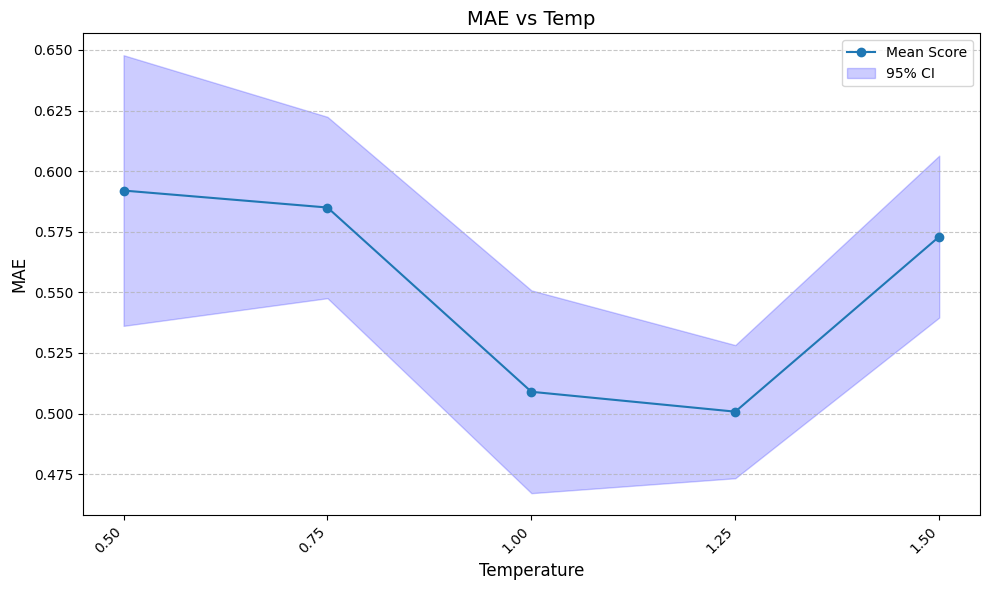
\includegraphics[width=0.9\linewidth]{temp_dependency.png}
    \caption{Mean Average Error on Big-Five traits set vs. Temperature parameter used for description generation. It c}
    \label{fig:enter-label}
\end{figure}
An important factor influencing the behavior of large language models during text generation is the \textit{temperature} parameter. Temperature controls the degree of randomness in the model’s output by scaling the probabilities of the next token in the sequence. Lower temperatures (e.g., 0.2–0.5) make the model more deterministic and focused, often favoring high-probability completions. In contrast, higher temperatures (e.g., 0.8–1.2) increase diversity by allowing less likely tokens to be sampled more frequently, resulting in more varied and creative—but also less predictable—outputs.

In the context of our framework, temperature plays a crucial role during the first stage, where the model generates a natural language \textit{description} based on a given set of personality trait scores. Since these descriptions serve as the input for subsequent trait inference, their fidelity to the original traits directly impacts the overall consistency score. A high temperature may lead to imaginative or stylistically rich descriptions that drift from the intended personality profile, while a low temperature may result in repetitive or overly rigid phrasing that underrepresents certain nuances of the personality.

To quantify the impact of temperature on descriptive consistency, we conducted several experiments using the Big Five personality traits. Each experiment varied the temperature parameter during the description-generation phase, and consisted of 200 runs to ensure statistical significance. We compared outcomes using Mean Absolute Error (MAE) between the original input scores and the scores inferred from the generated descriptions.

Our results indicate that intermediate temperatures (around 1.25) strike the best balance between expressiveness and trait fidelity. At this setting, descriptions are rich enough to reflect subtle trait cues while remaining grounded in the original score profile. Consequently, we adopted this temperature value for all subsequent experiments to ensure consistent and comparable evaluation across canonical and synthetic trait sets.

This result underscores an important insight: fidelity in reverse inference is not solely a function of linguistic precision or predictability. Rather, it depends on whether the generated text encodes enough semantically rich cues for the model to reconstruct the original intent. Temperature, in this sense, is not just a stylistic parameter—it plays a direct role in shaping how much of the latent trait signal is preserved in the text. We therefore adopt $T=1.25$ for all subsequent experiments to ensure consistency across both canonical and synthetic trait evaluations.

\section{Order Variation}
\begin{figure}[h]
    \centering
    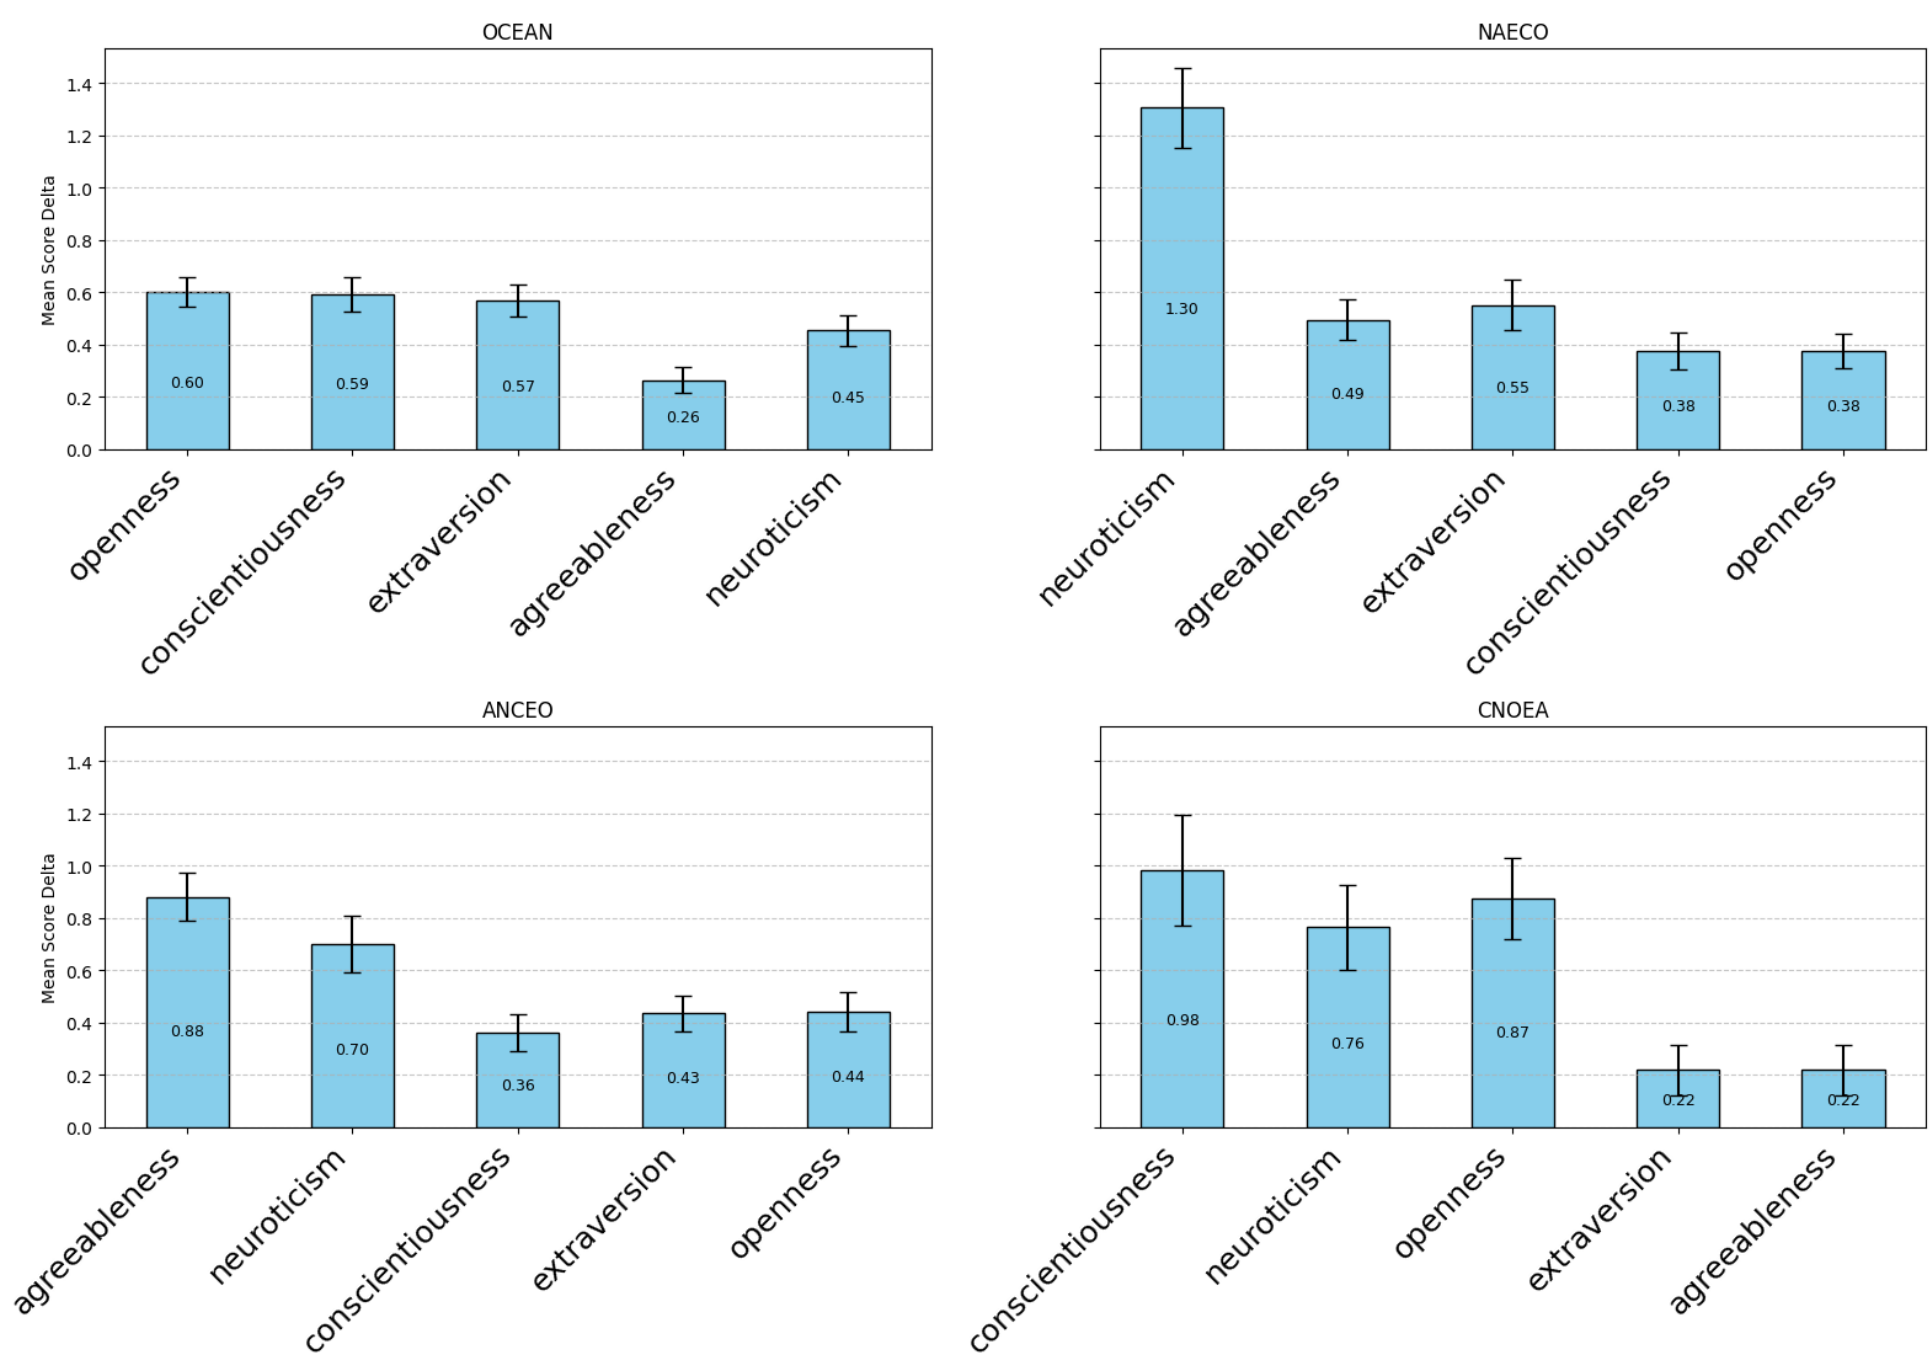
\includegraphics[width=0.9\linewidth]{order_exp.png}
    \caption{Mean Average Errors on Big-Five with different ordering of traits. In the top left corner is the most popular choice - OCEAN}
    \label{fig:enter-label}
\end{figure}
In our second experiment, we investigate the effect of trait ordering on LLM consistency, inspired by the findings of [\cite{gupta2023self}], who observed that LLM responses may vary depending on the sequence in which information is presented. To test this within our framework, we generate descriptions from the same set of Big Five personality scores, but vary the order in which traits are presented in the input prompt.

We evaluate four different orderings, including the canonical O-C-E-A-N sequence, as well as three alternative permutations. The inference step remains identical across conditions, using the generated description (from each ordering) to recover the original scores.

Our results show that trait order introduces major challenge when working with LLMs as they display different behaviour when presented with shuffled prompts. 


\section{Different Personality Dimensions}
\begin{figure}[h]
    \centering
    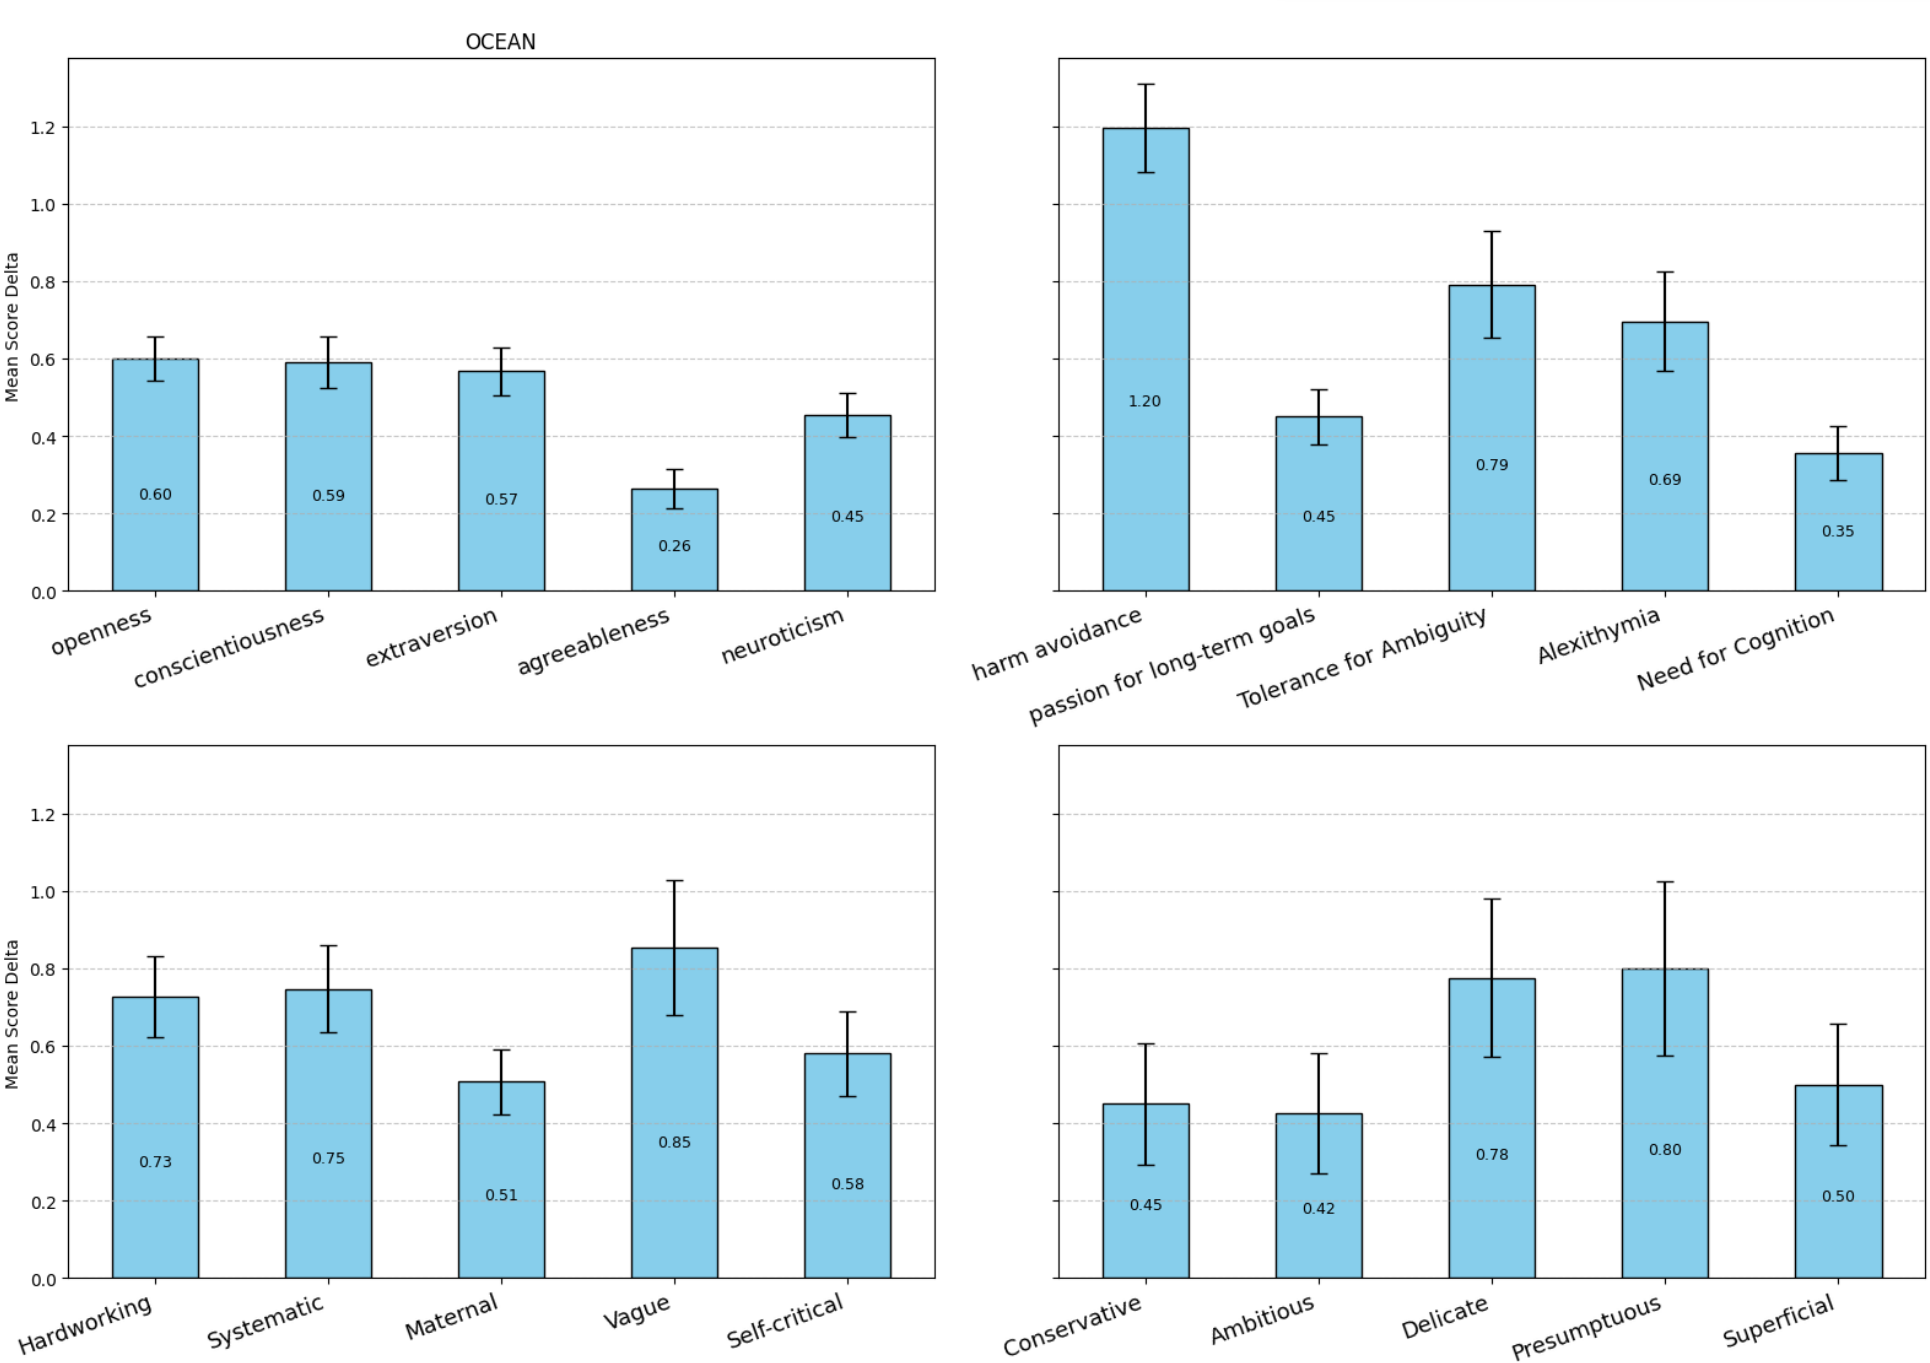
\includegraphics[width=0.9\linewidth]{diff_traits.png}
    \caption{Mean Average Errors on Big-Five with different ordering of traits. In the top left corner is the most popular choice - OCEAN}
    \label{fig:enter-label}
\end{figure}
In this experiment, we extend our evaluation beyond canonical personality constructs to include a variety of lesser-known or synthetic dimensions. While the Big Five model (OCEAN) serves as a well-established benchmark, real-world deployments often require LLMs to reason about personality traits that lack widespread theoretical grounding or consistent representation in training data. This experiment tests the adaptability and generalization of LLMs across such dimensions.

Figure4 presents the mean score deltas (original vs. inferred) for four different sets of traits. The top-left plot (OCEAN) provides a baseline, with most traits reconstructed with moderate accuracy (errors around 0.5–0.6), and agreeableness showing the highest fidelity (0.26). In contrast, the three alternative sets show more varied and often higher error rates.

The top-right plot includes constructs like \textit{harm avoidance} and \textit{alexithymia}, which are less commonly encountered in general discourse. Here, \textit{harm avoidance} exhibits a pronounced error (1.20), suggesting significant difficulty in encoding this trait from a textual description. Conversely, \textit{passion for long-term goals} and \textit{need for cognition} are inferred with relatively low error.

The bottom-left plot consists of more abstract or ambiguous constructs like \textit{vague}, \textit{maternal}, and \textit{self-critical}. Traits such as \textit{vague} result in higher errors (0.85), indicating interpretability challenges.

In the bottom-right plot, we present another synthetic trait set. Errors here remain moderate to high (up to 0.80), and standard deviations are often large, reflecting inconsistent reconstructions. This aligns with our broader observation that the less canonically defined or semantically diffuse a trait is, the more prone the LLM is to either misrepresent or default to stereotypical interpretations.

These results emphasize a key limitation: while LLMs can encode and reconstruct widely known personality traits with reasonable consistency, their generalization to non-canonical or synthetic dimensions is less reliable.

\section{Conclusion}

In this study, we introduced a novel two-stage framework to evaluate the consistency of Large Language Models (LLMs) in describing and scoring personality traits. By decoupling the processes of trait-to-text encoding and text-to-trait decoding across independent sessions, our methodology provides a robust, intrinsic benchmark for assessing LLMs' ability to simulate stable and coherent personalities. This framework advances the field by addressing key limitations of prior work, such as reliance on memorized associations and the narrow scope of predefined human-centric taxonomies.  

Our experiments revealed that LLMs exhibit higher consistency for well-established traits like the Big Five, while struggling with ambiguous or synthetic constructs. This underscores the tension between their flexible role-playing capabilities and their dependence on patterns embedded in training data. Additionally, we demonstrated the critical role of the temperature parameter in balancing expressive richness and trait fidelity, with intermediate values (e.g., 1.25) yielding the most reliable results. Trait ordering, had a significant impact on consistency.  

The development of this framework opens new avenues for research and application. It enables precise control over AI agent personalities, facilitating their use in simulations, virtual assistants, and other interactive systems where behavioral consistency is paramount. Future work could explore extensions to dynamic or context-dependent personality modeling, as well as the integration of multimodal inputs for richer trait representations.  

Ultimately, our findings highlight both the promise and limitations of LLMs in personality simulation, providing a foundation for more reliable and transparent AI agent design. The framework's adaptability to diverse trait sets positions it as a valuable tool for advancing the study of artificial personalities and their real-world applications.


\section{Limitations}
 First, our experiments were conducted exclusively using the DeepSeekV3 API. While this allowed for controlled and reproducible results, it limits the generalizability of our findings. Different LLMs (e.g., GPT-4, Claude, Gemini) may exhibit varying degrees of consistency due to differences in architecture, training data, and alignment techniques. Future work should expand evaluations to multiple models to assess whether our framework yields similar results across different systems.  
  

Additionally, our consistency metric relies on numerical reconstruction error, which may not fully capture semantic fidelity. A low error score does not necessarily mean the generated descriptions are contextually appropriate or nuanced. Human evaluations could complement automated metrics to assess qualitative aspects of personality simulation.  

Addressing these limitations in future work will strengthen the robustness and applicability of our framework, enabling more reliable profiling of LLM-based agents across diverse use cases.




\appendix

\section{Prompts} 
\textbf{Description prompt}\newline
Analyze the following personality description and provide numerical scores between 1 (low) and 5 (high) for each of these traits: <traits\_str>.

Description:
<description>

Format your response as a JSON dictionary with the trait names as keys (use lowercase) and the scores as values. Do not include any additional text or explanations.
Example response format:
<example\_json>\newline

\textbf{Scoring prompt}\newline
Create a detailed personality description matching these exact trait scores:
<traits\_with\_scores>

Express these traits however you like but you MUST NOT mention these scores as numbers explicitly. Your goal is to describe these scores in words in a best possible way
Critical constraints:
- Never reference numbers or scores in the description
- Avoid direct trait mentions (e.g., don't say 'extraverted')
- Show personality through specific, contextual details
- Maintain psychological plausibility
- Include nuanced contradictions when appropriate

%\nocite{*} % Includes all entries from the .bib file
\printbibliography % Correct command for biblatex
\end{document}